\section{BEAMER 模板}
\lstset{language={[LaTeX]TeX}}

\subsection{目录显示}
\index{命令!\verb$\tableofcontents$}

命令为:\\
\fbox{$\backslash$tableofcontents[用逗号分隔的选项]}

其中的主要选项有:\\

\begin{table}[htbp]
  \centering
  \caption{BEAMER 目录可选项}\label{contents}
\begin{tabularx}{14cm}{rX}
\toprule
  currentsection(或 currentsubsection) & 仅正常显示当前节(小节)目录,其他部分半透明 \\
  hideallsubsections & 不显示所有小节目录 \\
  hideothersubsections & 不显示当前节以外所有小节目录 \\
pausesections& 目录逐节显示,相当于每节目录后加上 $\backslash$pause 命令 \\
\bottomrule
\end{tabularx}
\end{table}

\subsection{创建帧}
\index{命令!\verb$\frame$}

\subsubsection{创建与结束}
\begin{lstlisting}[language={[LaTeX]TeX}]
\begin{frame}
\frametitle{...}
...
\end{frame}
`或`
\frame{...}
\end{lstlisting}

\subsubsection{颜色设置}
\index{命令!\verb$\beamersetaveragebackground$}

\begin{lstlisting}[language={[LaTeX]TeX}]
\beamersetaveragebackground{`颜色`}
\end{lstlisting}
用于设置帧背景的颜色\\
\verb$\alert{}$:将字体改为红色,强调用\\
\subsubsection{主题设置}

\index{命令!\verb$\useoutertheme$}
\index{命令!\verb$\useinnertheme$}
\index{命令!\verb$\usecolortheme$}
\index{命令!\verb$\usefonttheme$}
\index{命令!\verb$\usetheme$}


一共有五类主题,外部、内部、颜色、字体、演示。
\begin{lstlisting}[language={[LaTeX]TeX}]
\useoutertheme[`参数`]{`主题名`}
\useinnertheme[`参数`]{`主题名`}
\usecolortheme[`参数`]{`主题名`}
\usefonttheme[`参数`]{`主题名`}
\usetheme[`参数`]{`主题名`}
\end{lstlisting}

\begin{description}
  \item[外部主题] 设定上下边,导航条以及过渡样式

%%%%%%%%%%%%%%%%% 内部主题 %%%%%%%%%%%%%%%%%%%%%%%%%%%%%%%%
  \item[内部主题] 设定内部文本的常规列表(itemize)和排序列表(enumerate)格式及形状
  \begin{enumerate}
    \item default: 标记为小三角
    \item circles: (itemize)的标记改为小圆盘,(enumerate)添加背景圆盘,目录前加小圆盘
    \item rectangles: 跟上面一样,把标记变成方块
    \item rounded:同上,把标记变成圆球,模块背景框直角变圆弧,可选参数[shadow],可给 block 添加阴影。
  \end{enumerate}
%%%%%%%%%%%%%%%%%%%%%%%%%%%%%%%%%%%%%%%%%%%%%%%%%%%%%%%%%%%%%%%

  \item[颜色主题] 设定幻灯片颜色布局
  \item[字体主题] 设定标题,公式,文本,导航条的字体属性

%%%%%%%%%%%%%%%%% 演示主题 %%%%%%%%%%%%%%%%%%%%%%%%%%%%%%%
  \item[演示主题] 以上四种主题的组合排列主题名有下列 5 类:
\begin{enumerate}
  \item 无导航条:default
  \item 侧导航条:从上到下为题名简称,作者姓名,节标题和小节标题

  \begin{tabular}{ll}
    % after \\: \hline or \cline{col1-col2} \cline{col3-col4} ...
    Berkeley: & 左侧+符号条,蓝底白字 \\
    Goettingen: & 右侧+符号条,浅蓝底黑字 \\
    Hannover: & 左侧+符号条,浅蓝底黑字 \\
    Marburg: &  右侧+符号条,深蓝底白字\\
    PaloAlto: & 左侧+符号条,蓝底白字 \\
  \end{tabular}

  \item 顶边导航条
  \item 底边导航条
  \item 顶边+底边导航条
  \begin{itemize}
    \item AnnArbor: 顶边左段青底红字:节标题;右段黄底黑字,小节标题。
    底左蓝底红字,姓名院校;中黄底青字:题名简称;右日期帧码:黄底黑字。
    \item CambridgeUS: 同上,不同的是顶左褐底白字,右为灰底褐字。底左褐底白字,中灰底褐字,右灰底褐字
    \item Copenhagen:同上,底部只分两段,去除了日期和帧码,顶左黑底白字,右为蓝底白字。底左黑底白字,右蓝底白字
    \item Warsaw: 同 Copenhagen,在 block 外加了阴影,增加立体感
  \end{itemize}
\end{enumerate}
%%%%%%%%%%%%%%%%%%%%%%%%%%%%%%%%%%%%%%%%%%%%%%%%%%%%%%%%%%%%%%%

\end{description}


\subsubsection{加入时钟}

\index{命令!\verb$\initclock$}
\index{宏包!tdclock}

使用 tdclock 时钟宏包,\verb$\initclock$的时钟命令,如下所示
\begin{lstlisting}[language={[LaTeX]TeX}]
\usepackage[timeinterval=1]{tdclock}
\date[\initclock\tdtime]{\today}
\end{lstlisting}

\subsection{block 文本模块}
block 模块可以创建一个矩形区域,分标题和文本两块,用不同的颜色加以区别
\subsubsection{定理类}

包括定义、定理、证明、示例等环境(theorem、 definition、 lemma、 proof、 corollary、 problem)
显示的是带标题和文本两框的形式。用以下代码中文化,和引用。
\begin{lstlisting}[language={[LaTeX]TeX}]
\setbeamertemplate{theorems}[numbered]
`在定理后加数字,默认不加`
\begin{document}
\newtheorem{THeorem}{`定理`}
\newtheorem{DEfinition}{`定义`}
\newtheorem{PRoof}{`证明`}
\begin{theorem}
`文本框文字`
\end{theorem}
\begin{THeorem}
`文本框文字`
\end{THeorem}
\end{document}
\end{lstlisting}

\subsubsection{文本框}

\index{命令!\verb$\begin{block}$}
\index{命令!\verb$\begin{exampleblock}$}
\index{命令!\verb$\begin{alertblock}$}

有 block、exampleblock 和 alertblock 三种,用法如下:\\
\begin{lstlisting}[language={[LaTeX]TeX}]
\begin{block}{`标题栏文字`}
`文本框文字`
\end{block}
\end{lstlisting}

\subsubsection{文本盒子}

\index{beamer 环境!\verb$beamercolorbox$}
\index{beamer 环境!\verb$beamerboxesrounded$}

修饰文本的盒子环境,有彩色盒子环境 beamercolorbox 和圆角盒子环境 beamerboxesrounded 两种。
\begin{itemize}
  \item 彩色盒子:单独区域

\color{grass}
\begin{minipage}{12cm}
\verb$\begin{beamercolorbox}[参数]{beamer颜色}$\\
内容\\
\verb$\end{beamercolorbox}$
\end{minipage}
\normalcolor

其中参数的设置有:

\begin{tabular}{ll}
  wd=宽度 & 盒子宽度,默认为\verb$\textwidth$,文本行宽度 \\
  rounded=true & 盒子改为圆角 \\
  shadow=true & 增加阴影,当 rounded=true 时才有效 \\
  colsep=宽度 & 文本与盒子四边的距离 \\
  colsep$*$= & 文本与盒子上下边的距离 \\
  center & 文本与盒子水平居中对齐,默认为左对齐 \\
\end{tabular}

  \item 圆角盒子:包括标题区域和文本区域


\color{grass}
\begin{minipage}{12cm}
\verb$\begin{beamerboxesrounded}[参数]{标题}$\\
内容\\
\verb$\end{beamerboxesrounded}$
\end{minipage}
\normalcolor

\begin{tabular}{ll}
   width=宽度 & 盒子宽度 \\
  shadow=true & 增加阴影,当 rounded=true 时才有效 \\
  upper=beamer 颜色 & 标题区域的前景色与背景色 \\
  lower=beamer 颜色 & 文本区域的前景色与背景色 \\
\end{tabular}
\end{itemize}

\subsubsection{列表}

\index{beamer 命令!\verb$\setbeamercovered$}

主要两个命令进行控制逐幅显示
\begin{lstlisting}[language={[LaTeX]TeX}]
\setbeamercovered{transparent}%`逐幅显示的内容为半透明`
\begin{enumerate}
  \item `文本1`
  \pause
  \item `文本2`
\end{enumerate}
\end{lstlisting}


\subsection{分栏显示}
\subsubsection{minipage 环境实现多栏}
\index{环境!minipage}

可将幻灯片分为多栏,通常为 2 栏,如下所示:
\begin{lstlisting}[language={[LaTeX]TeX}]
\begin{minipage}[]{`宽度`}
\end{minipage}
\begin{minipage}[]{`宽度`}
\end{minipage}
\end{lstlisting}

对齐参数有:\\
\begin{tabular}{ll}

  b & 底行对齐 \\
  c & 中心对齐 \\
  t & 第一行对齐(基线) \\
  T & 第一行对齐(顶部) \\

\end{tabular}
\subsubsection{columns 环境实现多栏}
\index{beamer 命令!\verb$\column$}
可根据内部的 column 环境自动分栏。如下所示:
\begin{lstlisting}
\begin{columns}
\begin{column}[t]{5cm}
Two\\lines.
\end{column}
\begin{column}[t]{5cm}
Oneline(butaligned).
\end{column}
\end{columns}
% 或者
\begin{columns}
\column[t]{5cm}
Two\\lines.
\column[t]{5cm}
One line(but aligned).
\end{columns}
\end{lstlisting}

可选择项内参数有
\begin{itemize}
  \item b:底部对齐
  \item c:中心对齐
  \item t:顶部基线对齐
  \item T:顶部对齐
  \item onlytextwidth:相当于 totalwidth=\verb|\textwidth|
  \item totalwidth=\verb|{width}| :columns 默认是整幅帧宽度,可自定义宽度
\end{itemize}

\subsection{导航板设置}

\subsubsection{sidebar 参数设置}
\index{beamer 命令!\verb$\useoutertheme$}
共6个可选参数
\scriptsize
\begin{lstlisting}[language={[LaTeX]TeX}]
\useoutertheme[height=0.1\textwidth,width=0.15\textwidth,hideothersubsections,right]{sidebar} \end{lstlisting}
\normalsize
\begin{description}
  \item[height] 标题的高度
  \item[hideothersubsections]  显示所有的 subsection
  \item[hideallsubsections] 不显示subsections
  \item[left] 放在左边
  \item[right] 放在右边
  \item[width] sidebar 导航栏的宽度
\end{description}

\subsubsection{对应的目录导航有颜色显示}
\index{beamer 命令!\verb$\usecolortheme$}
使用如下主题
\begin{lstlisting}[language={[LaTeX]TeX}]
\usecolortheme{sidebartab}
\end{lstlisting}
\subsubsection{导航板logo设置}
\index{beamer 命令!\verb$\logo$}
\begin{lstlisting}[language={[LaTeX]TeX}]
\logo{\includegraphics[height=0.09\textwidth]{wuda.pdf}}
\end{lstlisting}

\subsection{时间设置}

\index{命令!\verb$\initclock$}
\index{宏包!tdclock}



下载 tdclock 宏包,用法如下:
\begin{lstlisting}[language={[LaTeX]TeX}]
\usepackage[`参数`]{tdclock}
\usepackage[timeduration=60,timewarningfirst=90,
timewarningsecond=95,colorwarningfirst=blue,
fillcolorwarningfirst=white!60!yellow,
fillcolorwarningsecond=white!10!yellow,timedeath=1]{tdclock}
\end{lstlisting}
\begin{tabular}{ll}
  timeinterval=n & n 秒更新一次 \\
  timeduration=n & n 分钟完成时间 \\
  timewarningfirst=n & 剩 n 秒后颜色变化默认90 (1-100)\\
  timewarningsecond=n & 剩 n 秒后颜色变化默认95 (1-100)\\
  colorwarningsecond=color  & 字体颜色 \\
  fillcolorwarningsecond=color & 背景颜色 \\
  timedeath=0or1 & 1为超过 110\%时间后关闭,0不关闭 \\
\end{tabular}



在之前须有\verb|\initclock|来进行时钟初始化,引用时间代码如下所示:\\
\begin{table}[ht]
\caption{引用时间对应代码} \centering
\rowcolors{2}{lightblue}{whiteblue}
\begin{tabular}{clcl}
\toprule
 % after \\: \hline or \cline{col1-col2} \cline{col3-col4} ...
时钟代码 & 对应时间 & 秒表代码 & 对应显示时间\\
  \verb|\tdclock| & 日期+时间 & \verb|\crono| & 时:分:秒 \\
  \verb|\tdtime| & 时间 & \verb|\cronohours| & 时 \\
  \verb|\tddate| & 日期 & \verb|\cronominutes| & 分 \\
  \verb|\tdday| & 日 &  \verb|\cronoseconds| & 秒  \\
  \verb|\tdmonth| & 月 & \verb|\resetcrono{"button"}| & 复位秒表 \\
  \verb|\tdyear| & 年 & \verb|\toggleclock{"button"}|& 秒表、时钟切换\\
  \verb|\tdhours| & 时 && \\
  \verb|\tdminutes| & 分 && \\
  \verb|\tdseconds| & 秒 && \\
  \bottomrule
\end{tabular}
\end{table}
~\\
PDF 样例参考 \ref{texref}\\


\subsection{加入附件}

\index{命令!\verb$\textattachfile$}
\index{命令!\verb$\attachfile$}
\index{命令!\verb$\notextattachfile$}
\index{命令!\verb$\noattachfile$}

使用 attachfile2 宏包,可加入真 3d pdf,MS 的 word,excel等,可双击直接打开。
但压缩文件 rar 类型不能从附件中下载,可将 RAR 的压缩文件后缀改成 ar ,
从 pdf 的附件下载后再将后缀改为 rar 类型即可。

引用代码:
\begin{lstlisting}[language={[LaTeX]TeX}]
\usepackage{attachfile2}
`四种引用方式`
\textattachfile{`附件名称`}{`显示图片或文字`}
\attachfile[icon=`图标名称`]{`附件名称`}
`以下两种只显示名称,不加入附件`
\notextattachfile{`附件名称`}{`显示图片或文字`}
\noattachfile[icon=`图标名称`]{`附件名称`}
\end{lstlisting}

icon= 有四种参数,如下图所示:

\begin{figure}[htbp]%位置选项
\centering
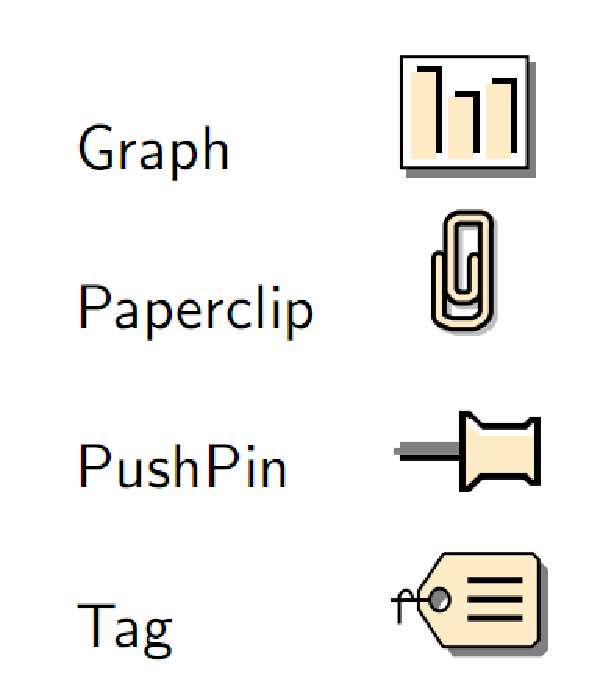
\includegraphics[width=4cm]{icon.pdf}
\caption{附件显示图标} \label{icon}
\end{figure}


\subsection{遮盖,逐步显示}

\subsubsection{遮盖命令}
\index{命令!\verb$\pause$}
\index{命令!\verb$\uncover$}
\index{命令!\verb$\only$}
\index{命令!\verb$\alt$}
\index{命令!\verb$\visible$}
用以下命令可以实现遮盖的效果。
\begin{itemize}
  \item \verb|\pause|:
  \item \verb|\uncover|:
  \item \verb|\only<n->|:只在第 n 张中显示
  \item \verb|\alt|:变换命令
\end{itemize}
对应命令 \verb|\only,\alt,\visible,\uncover,\invisible|有相应的环境 onlyenv, altenv, visibleenv, uncoverenv, invisibleenv,在环境中的元素相当于加入了命令。

\index{环境!overylayarea}
在前后两张 slide 中的同一位置实现内容的改变可用 overlayarea 环境。这样后一张 slide 的内容出现位置会在前一张设定的区域内
\begin{cmd}
\begin{overlayarea}{area width}{area height}
environment contents
\end{overlayarea}
 example:
\begin{frame}
\begin{overlayarea}{\textwidth}{3cm}
\only<1>{Some text for the first slide.\\Possibly several lines long.}
\only<2>{Replacement on the second slide.}
\end{overlayarea}
\end{frame}
\end{cmd}

\subsubsection{表格逐列显示}

\index{命令!\verb$\onslide<n->stuff$}

\verb|\onslide<n->stuff|命令,代码如下表所示:
\begin{shaded}
\begin{Verbatim}
\begin{tabular}{l!{\vrule}c<{\onslide<2->}c<{\onslide<3->}%
c<{\onslide<4->}c<{\onslide}c}
Class & A & B & C & D\\
X & 1 & 2 & 3 & 4\\
Y & 3 & 4 & 5 & 6\\
Z & 5 & 6 & 7 & 8
\end{tabular}
\end{Verbatim}
\end{shaded}
\subsubsection{列表逐项显示}

\index{命令!\verb$\item<n->$}
\index{命令!\verb$\item<+->$}

\begin{shaded}
\begin{Verbatim}
\item<n->  : n 表示从第 n 张开始显示
<+->    : 自动逐项显示
\item<n1-n2>    : 手动控制显示顺序
\end{Verbatim}
\end{shaded}

效果如下,双击显示\footnote{建议用 Adobe Reader 9 以上阅读器}:\\
\begin{enumerate}
  \item  \textcolor[rgb]{1.00,0.00,0.00}{手动控制逐步显示 }\\~\\
\textattachfile{stepview1.pdf}{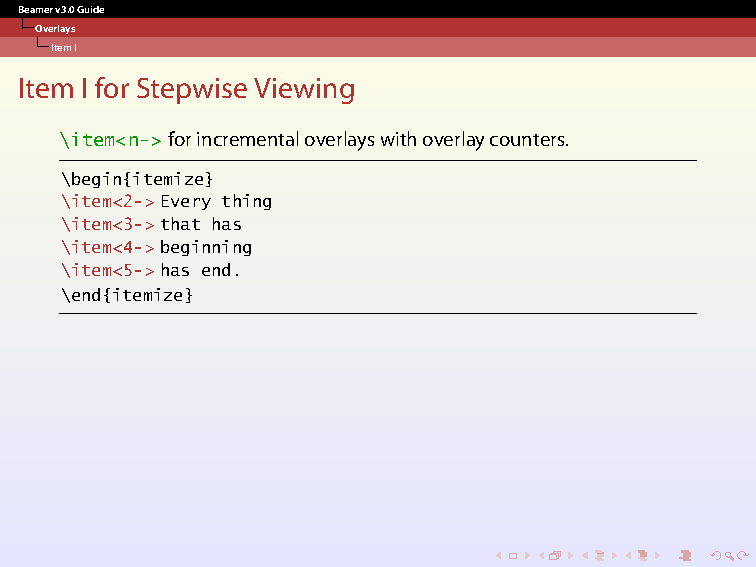
\includegraphics[width=10cm]{body/stepview1_face.pdf}}\\
  \item \textcolor[rgb]{1.00,0.00,0.00}{自动控制逐步显示}\\~\\
\textattachfile{stepview2.pdf}{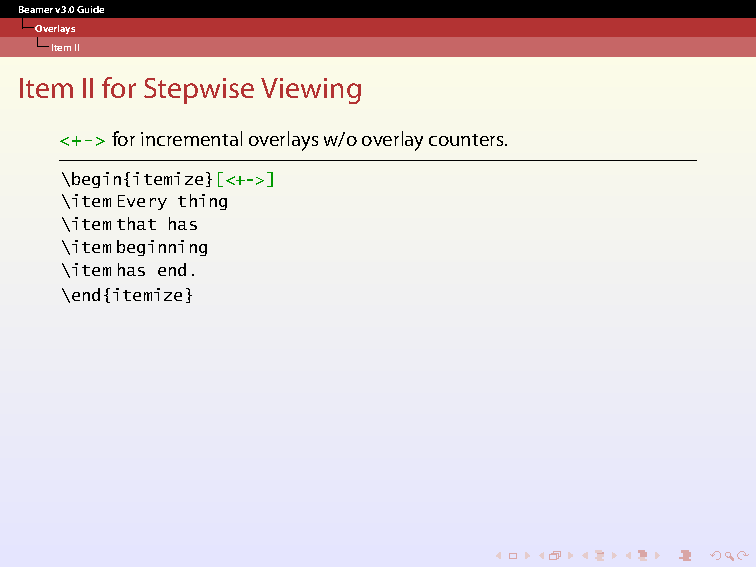
\includegraphics[width=10cm]{body/stepview2_face.pdf}}\\
  \item \textcolor[rgb]{1.00,0.00,0.00}{手动控制跳跃显示}\\~\\
\textattachfile{stepview3.pdf}{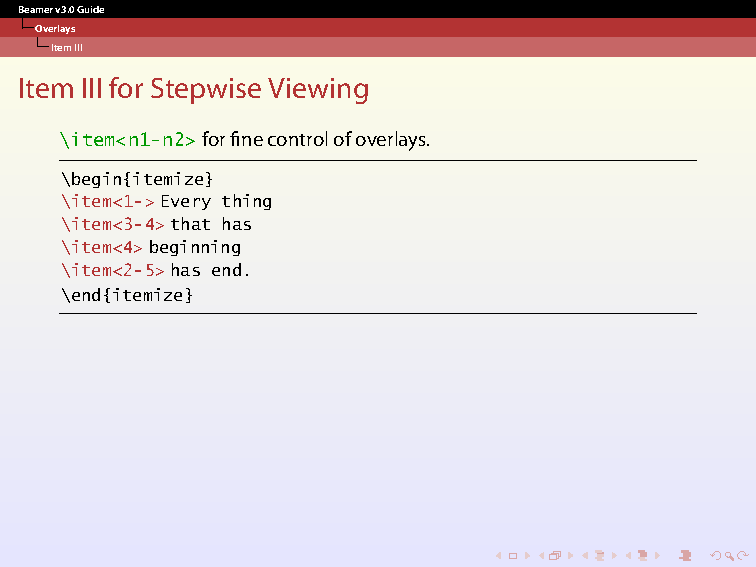
\includegraphics[width=10cm]{body/stepview3_face.pdf}}\\
\end{enumerate}

\subsubsection{内容逐项变化}

\index{命令!\verb$\only<n>$}
\index{命令!\verb$\uncover<n>$}
\index{命令!\verb$\invisible<n>$}
\index{命令!\verb$\alt<n>$}
\index{命令!\verb$\temporal<n>$}

\begin{shaded}
\begin{Verbatim}
\only<n>{..}
在第n张显示括号内的内容,连续性显示。
\uncover<n>{..}
只在第n张显示括号内的内容
\invisible<n>{..}
只在第n张内隐藏括号内的内容
\alt<n>{内容1}{内容2}
在第n张显示内容1,其它张显示内容2
\temporal<n>{内容1}{内容2}{内容3}
第n张前显示内容1,第n张显示内容2,第n张后显示内容3
\end{Verbatim}
\end{shaded}
\textcolor[rgb]{1.00,0.00,0.00}{效果如下所示}\\~\\
\textattachfile{replace1.pdf}{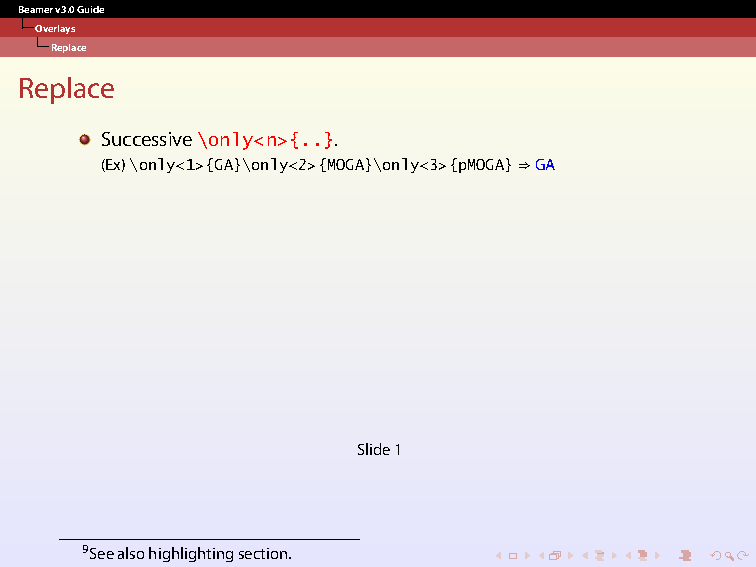
\includegraphics[width=10cm]{body/replace1_face.pdf}}\\
\subsubsection{列表逐项高亮变色}
有四种方案:\\

\index{命令!\verb$\item <+-| alert@+>$}

\begin{enumerate}
  \item \textcolor[rgb]{1.00,0.00,0.00}{从无到有的高亮}\\~\\
\textattachfile{highlight1.pdf}{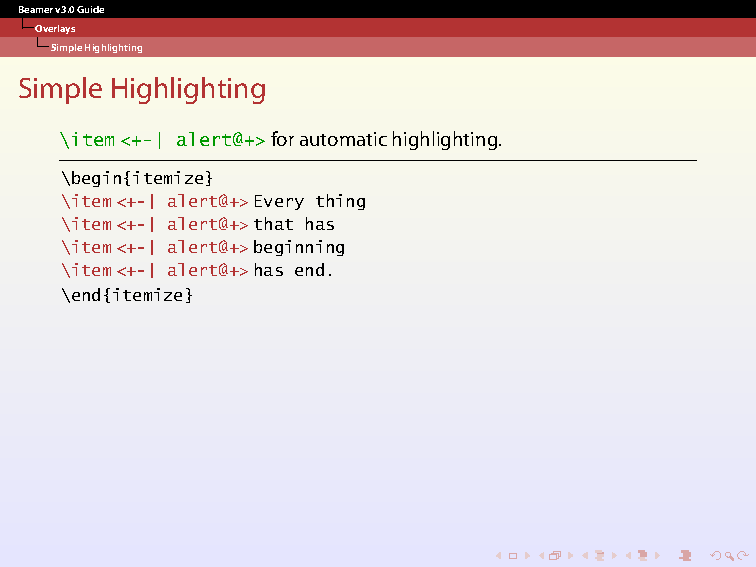
\includegraphics[width=10cm]{body/highlight1_face.pdf}}\\
\begin{shaded}
\begin{Verbatim}
\begin{itemize}[<+-|alert@+>]
以上为自动逐项高亮
\item <+-| alert@+>
以上为手动为每项加高亮
\end{Verbatim}
\end{shaded}


  \item \textcolor[rgb]{1.00,0.00,0.00}{全显示逐步高亮}\\~\\


\index{命令!\verb$\item<2-| alert@2>$}

  \textattachfile{highlight2.pdf}{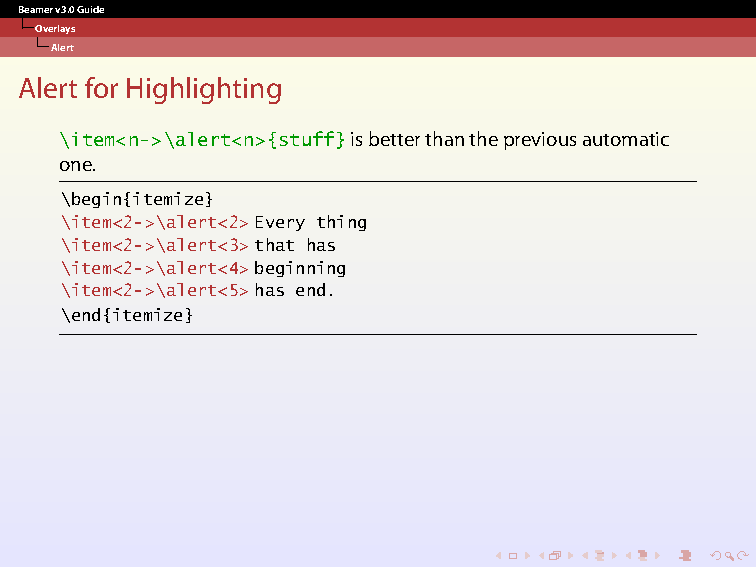
\includegraphics[width=10cm]{body/highlight2_face.pdf}}\\
\begin{shaded}
\begin{Verbatim}
\item<n->\alert<n>{stuff}
第n张显示高亮
\item<2->\alert<2>
\item<2-| alert@2>
以上两种效果相同
\end{Verbatim}
\end{shaded}

  \item \textcolor[rgb]{1.00,0.00,0.00}{可配置底色高亮}\\~\\

\index{命令!\verb$\alt<n>$}

  \textattachfile{highlight3.pdf}{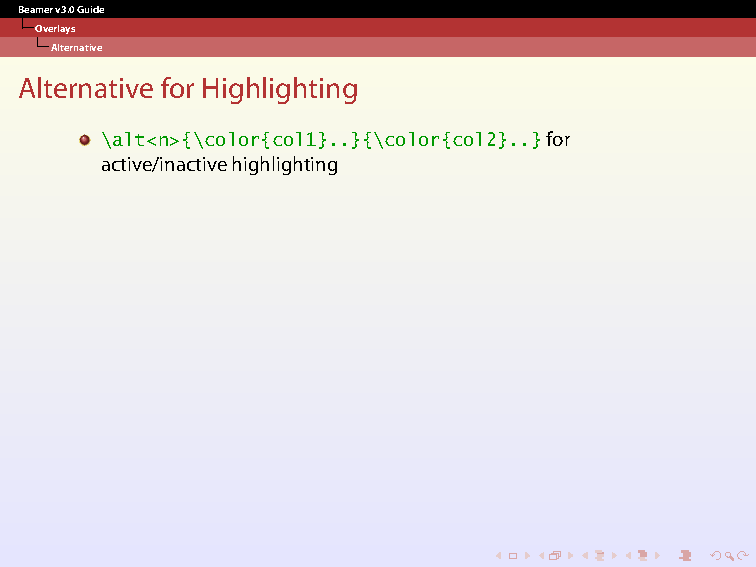
\includegraphics[width=10cm]{body/highlight3_face.pdf}}\\
\begin{shaded}
\begin{Verbatim}
\alt<n>{\color{col1}..}{\color{col2}..}
前面的括号是高亮时的颜色和内容,后面是不高亮时的颜色和内容
\end{Verbatim}
\end{shaded}

  \item \textcolor[rgb]{1.00,0.00,0.00}{高亮后底色变化}\\~\\

\index{命令!\verb$\temporal<n>$}

  \textattachfile{highlight4.pdf}{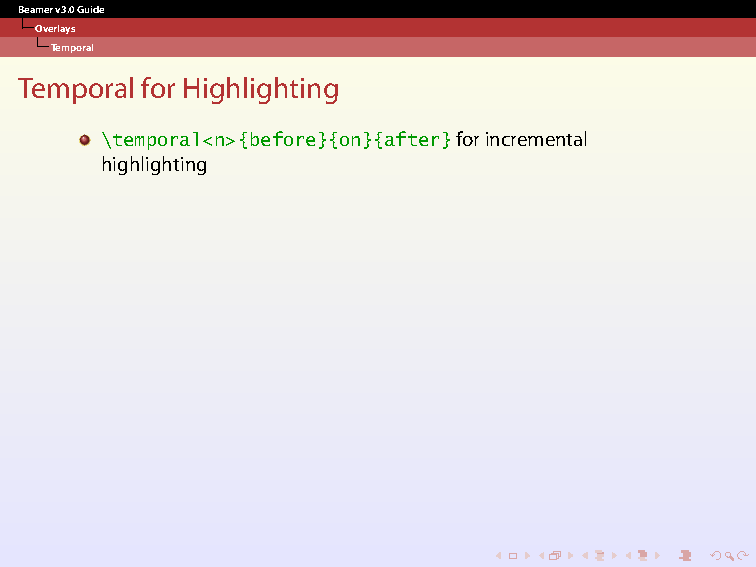
\includegraphics[width=10cm]{body/highlight4_face.pdf}}\\
\begin{shaded}
\begin{Verbatim}
\def\hilite<#1>{%
\temporal<#1>{\color{gray}}{\color{blue}}%
{\color{blue!25}}}
...
\temporal<n>{before}{on}{after}
before 为高亮前颜色,on 为高亮颜色,after 为高亮后颜色。

\end{Verbatim}
\end{shaded}
\end{enumerate}



%%%%%%%%%%%%%%%%%%%%%%%%%%%%%%%%%%%%%%%%%%%%%%%%%%%%%%%%%%%%
\subsection{代码抄录 semiverbatim lstlisting}
可用 verbatim 和 lstlisting 环境,semiverbatim 环境类似于 verbatim ,但里面的 \verb|\,{,}| 符号保持原意,在 semiverbatim 环境中可用 \verb|\\,\{,\}| 来表示原符号。使用以上环境时必须在\verb|\begin{frame}|后加上可选项 fragile。\verb|\begin{frame}[fragile]|。

%%%%%%%%%%%%%%%%%%%%%%%%%%%%%%%%%%%%%%%%%%%%%%%%%%%%%%%%%%%%
\subsection{切换颜色}


beamer 颜色由三类构成:
\begin{itemize}
  \item Navigational bars
  \item Background
  \item Structure
\end{itemize}
\subsubsection{定义新颜色}
\begin{shaded}
\begin{Verbatim}
颜色1!百分比1!颜色2
%颜色2占有剩下的百分比
green!80!gray
%表示80%green加20%gray
-green
%表示从以前的颜色移除green
\end{Verbatim}
\end{shaded}
\subsubsection{改变 alert 颜色}
如\ref{alert change}所示

\begin{figure}[H]
  \centering
  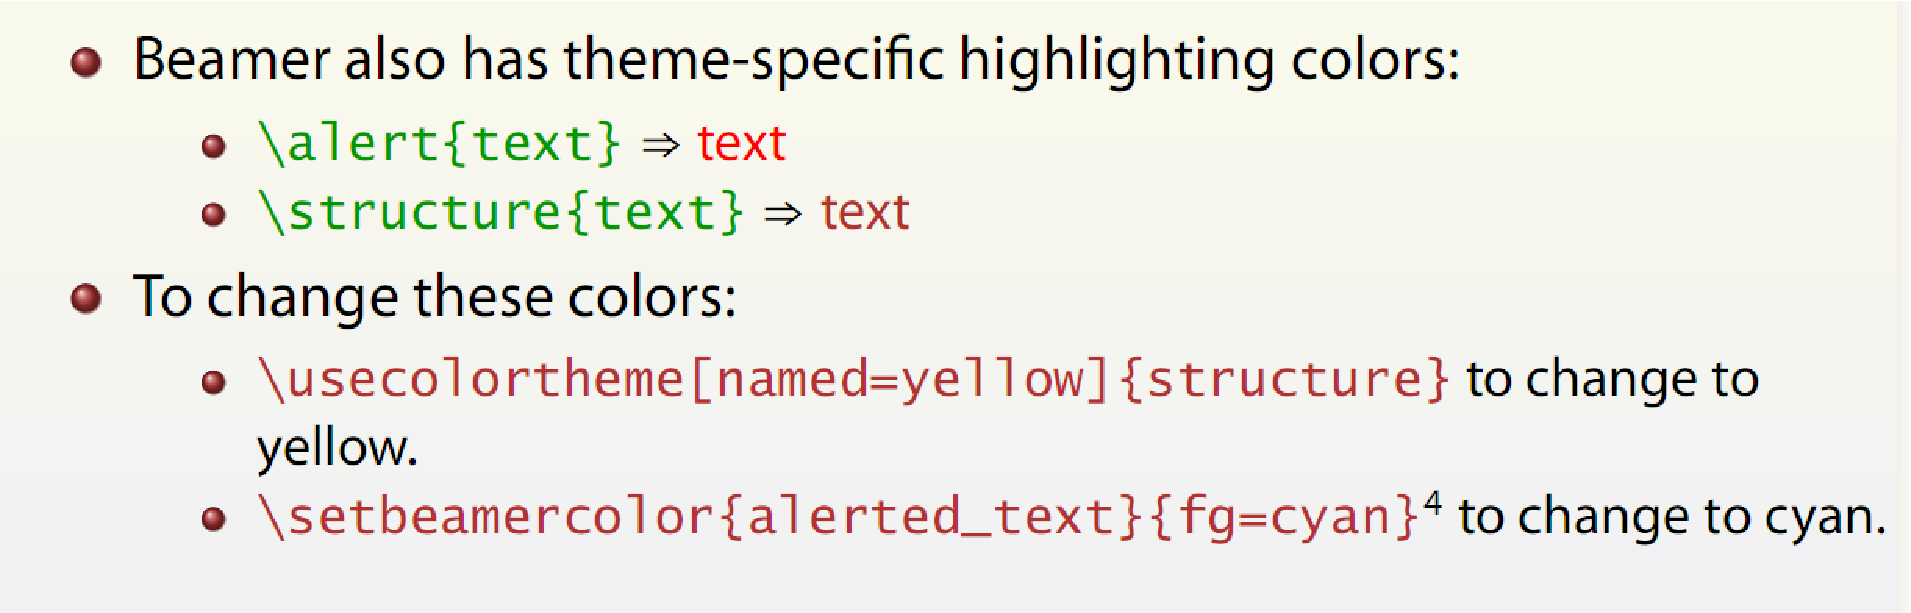
\includegraphics[width=12cm]{coloralertstructure}\\
  \caption{改变 alert 颜色}\label{alert change}
\end{figure}
\subsubsection{改变 background 颜色}

\index{命令!\verb$\beamersetaveragebackground$}
\index{命令!\verb$\beamertemplatesolidbackgroundcolor$}
\index{命令!\verb$\beamertemplateshadingbackground$}
\index{命令!\verb$\beamertemplategridbackground$}

有实体、倾斜、格点三种颜色模式。
\begin{shaded}
\begin{Verbatim}
%soild颜色
\beamersetaveragebackground{color} or
\beamertemplatesolidbackgroundcolor{color}
%gradient颜色
\beamertemplateshadingbackground{color1}{color2}.
% The colors in this slide is {blue!5}{yellow!10}.
%grid颜色
\beamertemplategridbackground[grid_space].
\end{Verbatim}
\end{shaded}
\subsubsection{改变 structure 颜色}


\index{命令!\verb$\colorlet$}
\index{命令!\verb$\usestructuretemplate$}
\index{命令!\verb$\beamertemplateshadingbackground$}

\begin{shaded}
\begin{Verbatim}
\colorlet{mystruct}{structure}%Save current structure
\colorlet{structure}{magenta}%New structure
\usestructuretemplate{\color{structure}}{}%\structure{..}
\beamertemplateshadingbackground{yellow!50}{magenta!50}
%New background
\frame{%
...
}%
%Back to the original "structure" and bgcolor schemes
\colorlet{structure}{mystruct}
\beamertemplateshadingbackground{blue!10}{yellow!10}
\end{Verbatim}
\end{shaded}


\subsection{带进度条的幻灯片}
如下图所示:
\begin{figure}[H]
  % Requires \usepackage{graphicx}
\centering
  
\includegraphics[width=12cm]{nav_beamer}\\
  \caption{带进度条的 BEAMER 幻灯片}\label{nav_beamer}
\end{figure}

需把 beamerouterthemeprogressbar.sty 文件放在同一文件夹下,在 BEAMER 的  tex 文件中加入:
\begin{cmd}
  \useoutertheme{progressbar}
\end{cmd}
注意原网络上下载的宏包有错误,须将其代码进行更正后方能编译成功。附件中为已更正的宏包。原宏包更改方式为:
把宏包中的代码:
\begin{lstlisting}
\draw (\progressbar@leftbar, 0.11cm)
[draw=bg!70!fg, rounded corners=0.1cm]
rectangle ++(\progressbar@barlength mm, 0.2cm);
\end{lstlisting}
替换成下面的代码:
\begin{lstlisting}
\draw (\progressbar@leftbar, 0.11cm)
[draw=bg!70!fg, rounded corners=0.1cm]
rectangle ++(\progressbar@barlength*.1cm, 0.2cm);
\end{lstlisting}
即可。

\subsection{note 添加笔记}

可以用来给 beamer 增加讲义,可将讲义单独输出,或混合输出各种方式。
\begin{cmd}
\note{text} % 使用方式
\setbeameroption{show notes} % include notes and normal text
\setbeameroption{hide notes} % default, hide notes page
\setbeameroption{show only notes} % output only notes page
\setbeameroption{show notes on second screen={location} % left,bottom,top
\end{cmd}



